\RequirePackage{lineno}  % http://www-d0.fnal.gov/Run2Physics/WWW/templates/lineno.html
%\documentclass[12pt]{iopart}
\documentclass[11pt, titlepage]{article}
\usepackage[top=20mm, bottom=20mm, left=23mm, right=23mm]{geometry}
%\newcommand{\gguide}{{\it Preparing graphics for IOP journals}}
%Uncomment next line if AMS fonts required
%\usepackage{iopams}  
% parameters from other files
\newcommand{\citetapos}[1]{\citeauthor{#1}'s \citeyearpar{#1}}  % apostrophe's in cites
%\usepackage[square,numbers,sort&compress]{natbib}
\def\linenumberfont{\normalfont\small\sffamily}
\usepackage{graphicx}
\usepackage{epstopdf}
% From link below: next two lines allow caption to fill the full figure box, and caption formats to be changed (e.g. font)
% http://tex.stackexchange.com/questions/107350/caption-below-the-figure-and-aligned-with-left-side-of-figure
% http://ctan.mackichan.com/macros/latex/contrib/caption/caption-eng.pdf
\usepackage{caption}
\captionsetup[figure]{slc=off, font=footnotesize}
%\usepackage{amsmath}
\usepackage{longtable}
\usepackage{placeins}
\usepackage{multirow}
\usepackage[numbers,round,sort,compress]{natbib}
\bibpunct{(}{)}{,}{n}{,}{,}  % https://xianblog.wordpress.com/tag/natbib/ (allows natbib with PNAS)
% figures float at top of page
\makeatletter
\setlength{\@fptop}{0pt}
\setlength{\@fpbot}{0pt plus 1fil}
\makeatother

\begin{document}
%\bibliographystyle{unsrt}

\setpagewiselinenumbers
%\modulolinenumbers[5]
%\linenumbers
\begin{center}\section*{\Large Supplementary Methods and Results}\end{center}
%\begin{table}[ht]
%\centering
%\caption{Confidence classes for the forcing data based on bias-correction weights.}
%\begin{tabular}{cc}
%  \hline
%  Confidence class & Bias-correction weight \\ 
%  \hline
%High & 0.75-1.00 \\ 
%Medium-High & 0.50-0.75\\ 
%Medium-Low & 0.25-0.50\\ 
% Low & 0.05-0.25 \\ 
% None & $<$0.05 \\ 
%   \hline
%\end{tabular}
%\end{table}  
\section{\large Overview}
This document provides supplementary information on methods and results from the different components of the analysis described in the main text.  The code used to conduct the analysis is presented after sections 1-X.  

\section{\large Reference data accuracy}

The accuracy of the reference vector dataset was assessed by Estes et al \cite{estes_platform_2015}, and described further here. The assessment was undertaken using a sub-sample of 609 1 km$^2$ grid cells, which were selected using a weighted randomized sampling scheme. Weights were derived from a logistic regression model of cropland occurrence probability in South Africa, with 1 corresponding to the lowest quartile of probability, and 4 the highest. The accuracy assessment included all cropland classes mapped within the reference dataset, which ranged from communal/smallholder fields to commercial row crops to orchards and other types of horticulture. A visual accuracy assessment was conducted within each 1 km$^2$ grid cell, wherein each cell was divided into 25 smaller cells of 200 X 200 m (4 ha), and then the proportion of each cell overlapping with cropfields visible in underlying, high resolution Google Maps imagery was then calculated to the nearest 5\% of coverage, using a finer 20-cell mesh overlaid on each sub-cell within which field presence/absence was recorded. The same procedure was then performed to assess coverage by reference map polygons, as well as the intersections and differences between cells determined to be occupied by i) visual assessment and ii) by the digitized polygons. These intersections and differences were used to calculate the area of true positives, false positives, true negatives, and false negatives within each 1 km$^2$ grid cell, which were then used to calculate accuracy measures.  In this case, accuracy was assessed using two landcover classes: cropland and non-cropland, thus a two class confusion matrix was constructed (Table 1) according to remote sensing classification accuracy guidelines set out by Oloffson et al. \cite{olofsson_good_2014}. In this case, the reference data were the visually interpreted crop field presences/absences, and the map data were the field boundary vectors being assessed (i.e. the data which provide the reference maps in this study), the class ``crop" refers to crop field presence and ``non-crop" to crop field absence.  The total area of vectorized crop fields was used to calculate the proportion \emph{W} of South Africa's total area mapped as crop fields, and of the areas ``mapped'' (by omission) as having other cover types.  These were then used to weight the proportions of each mapped class \emph{i} corresponding to each reference class \emph{j} by the total area \emph{A} mapped for class \emph{i}. The total accuracy (0.97, or 97\%) was calculated by summing the diagonal (bold in Table 1), as well as the producer's accuracy \emph{P} for each reference class \emph{j}, and the user's accuracy \emph{U} for each mapped class \emph{i}.  

\begin{table}[!ht]
\centering
\caption{Confusion matrix for the assessment of the hand-digitized crop field boundaries used to generate reference cropland cover percentage values. Here \emph{Reference} denotes a visual assessment of crop field presence in high resolution imagery within a sample of 609 sites, while \emph{Map} refers to the vectorized crop field boundaries. The assessment had two classes: crop fields and non-crop fields, and proportions corresponding to these two categories are the proportions of areas determined by class agreements and disagreement in the 609 sites (see text above), which are weighted by the proportion \emph{W} of each class' total mapped area \emph{A$_i$} in South Africa. \emph{P} and \emph{U} provide the Producer's and User's accuracies, respectively. }
\begin{tabular}{rrrrrrr}
  \hline
  & & Reference (j) & & & & \\\cline{3-7}
  & & Crop & Non-crop & \emph{W}$_i$ & \emph{A}$_i$ (ha) & \emph{U}$_i$ \\ 
  \hline
  Map (i) & Crop & \textbf{0.108} & 0.007 & 0.114 & 14018567 & 0.943 \\ 
  & Non-crop & 0.021 & \textbf{0.865} & 0.886 & 108541733 & 0.977 \\ 
  & Total & 0.128 & 0.872 & 1.000 & 122560300 &  \\ 
  & \emph{P}$_j$ & 0.840 & 0.992 &  &  &  \\ 
   \hline
\end{tabular}
\end{table}

%\clearpage
\FloatBarrier
\section{\large Cropland map error analysis}
We examined the impact of several sources of uncertainty on our results.  The first is the potential temporal mismatch between the reference dataset and the landcover products we were testing.  We tested this by examining two versions of the reference dataset, the initial version created in 2007, and the updated version from 2011 used in the main analysis.  The 2011 version shows 3\% more cropland area than the 2007 version. To examine the effect of the over mapping bias and accuracy measures, we converted the 2007 vector maps to gridded cropland percentage and subtracted each test map, and then compared the differences in bias and mean absolute error (MAE) values calculated between both (Table 2). The largest difference was 1.63\%, between the 1 km SA-LC residuals, which means that the overestimation bias by SA-LC was actually greater relative to the 2007 version of the reference map.  Except for the corresponding MAE value, all other difference were $<$1\%. 

% latex table generated in R 3.2.1 by xtable 1.7-4 package
% Wed Nov 25 15:57:07 2015
\begin{table}[!ht]
\caption{Differences in the bias and mean absolute errors values resulting from cropland percentage residuals calculated using 1) the 2011 reference map and 2) the 2007 reference map, with 2007 values subtracted from 2011 values. Differences from each test map and each scale of aggregation are shown. }
\centering
\begin{tabular}{rlrrrr}
  \hline
 & Resolution & SA-LC & GlobCover & MODIS & GeoWiki \\ 
  \hline
1 & 1 km & 1.63 & -0.80 & 0.12 & 0.64 \\ 
  2 & 5 km & 0.99 & -0.38 & 0.40 & 0.80 \\ 
  3 & 10 km & 0.89 & -0.27 & 0.44 & 0.77 \\ 
  4 & 25 km & 0.83 & -0.12 & 0.47 & 0.76 \\ 
  5 & 50 km & 0.79 & 0.04 & 0.47 & 0.73 \\ 
  6 & 100 km & 0.76 & 0.19 & 0.54 & 0.72 \\ 
  7 & 1 km & 1.30 & -0.77 & -0.10 & 0.27 \\ 
  8 & 5 km & -0.22 & -0.44 & -0.08 & 0.12 \\ 
  9 & 10 km & -0.48 & -0.34 & -0.08 & 0.12 \\ 
  10 & 25 km & -0.61 & -0.20 & -0.08 & 0.20 \\ 
  11 & 50 km & -0.67 & -0.09 & -0.36 & 0.22 \\ 
  12 & 100 km & -0.70 & 0.04 & -0.24 & 0.19 \\ 
   \hline
\end{tabular}
\end{table}

As a further exploration of uncertainty, we included the full range of variability that resulted from a) using either the 2007 or 2011 map to calculate bias and accuracy, and b) from different levels of cropland percentages used when converting MODIS and GlobCover mixed cropland classes into cropland percentage maps, following Fritz et al. \cite{fritz_mapping_2015}. We pooled the residuals from across each of these permutations, for each reference-test map combination, and examined how their overall mean values change with aggregation scale (Fig. 1), and also assessed the total distribution of errors within different class of cropland density, determined by dividing the 2011 1 km reference map into 20 different zones, or bins, of cropland density, ranging from 0-5\% cropland cover up to 95-100\% cover. We then calculated summary statistics from the pooled residuals and absolute values of residuals within each of these bins (Fig. 2).   

\begin{figure}[!ht]
  \centering
     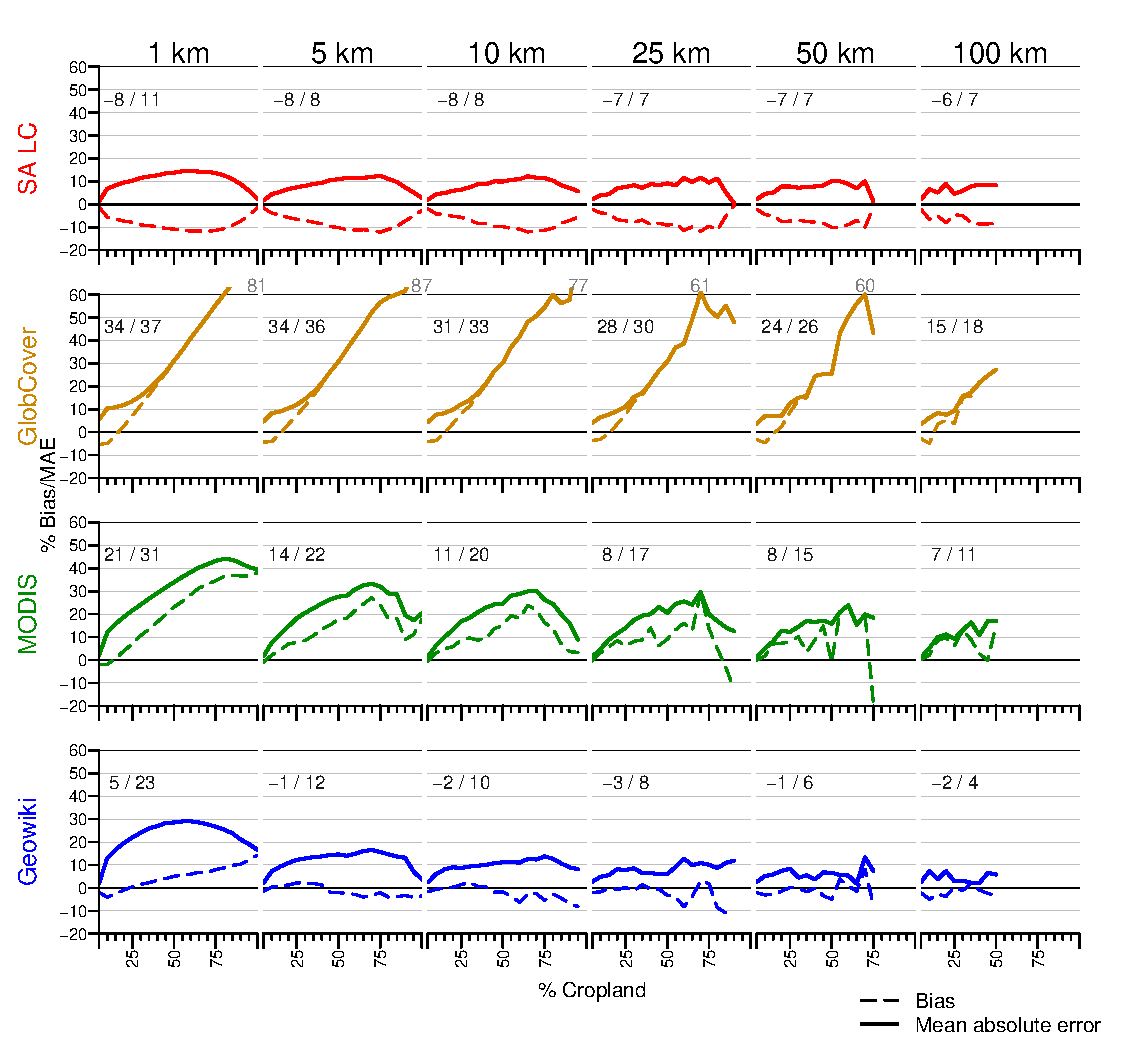
\includegraphics[width = 14cm]{figures/biases_1-100km.pdf} 
%     \vspace{-3cm}
      \caption{Biases and mean absolute errors (MAE) for each of the cropland maps as a function of cropland density (calculated using the 2011 reference maps) and aggregation scales. Rows present biases by map product, columns by aggregation scale.  Dash lines indicate bias at each level of cropland density, calculated in bins spanning 5\% of density (e.g. 0-5\% cropland cover, 5-10\%, etc.), while solid lines indicate the mean absolute error.  The black numbers in each plot area present the overall means of bias/MAE for each sensor-scale combination. The bin-wise and overall mean statistics were calculated from pooled map errors calculated from differences between the 2007 reference map and each cropland map (including all three variants--high, medium, and low--of the MODIS and GlobCover-derived cropland maps), and the 2011 reference map and each cropland map. }
      \label{fig:default}
\end{figure}

%\vspace{0.5 cm}
%\begin{equation}
%\hspace*{1.5 cm} 
%   \label{metric}
%     R_n  = \frac{(1 - \alpha)dswr + dlwr - \sigma * T^4}{\lambda}
%\end{equation}

\begin{figure}[!ht]
  \centering
     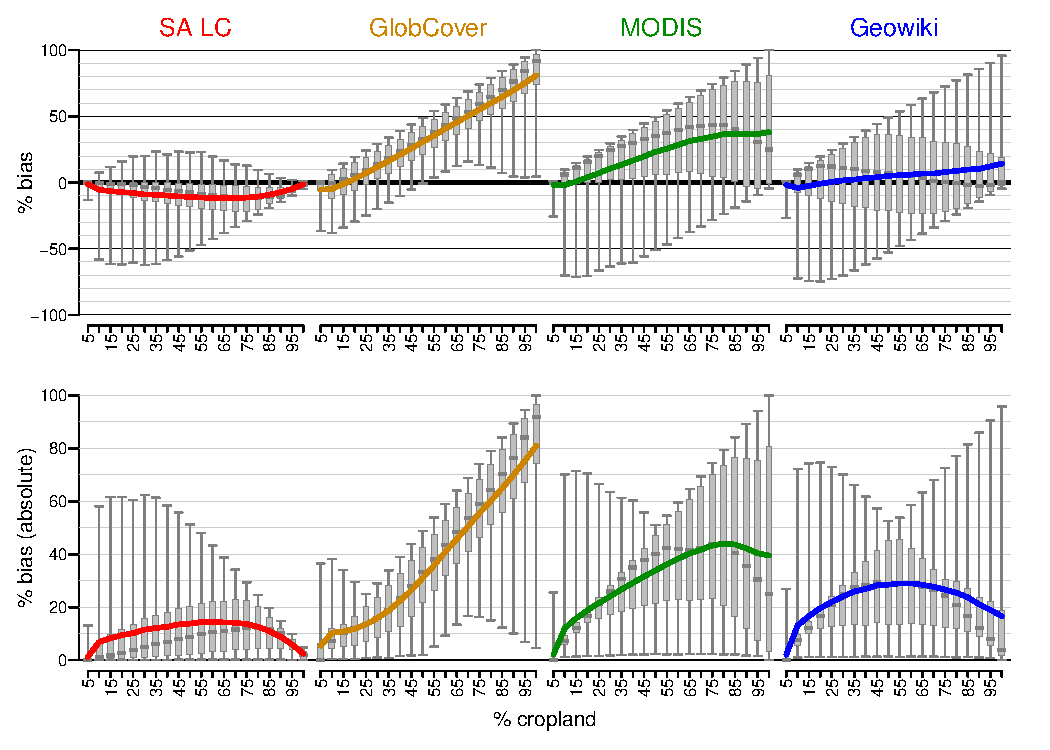
\includegraphics[width = 14cm]{figures/biases_1km.pdf} 
%     \vspace{-3cm}
      \caption{Biases and mean absolute errors (MAE) for each of the cropland maps at 1 km resolution, as a function of cropland density. Colored lines (color-coded to map product name) show the bias/MAE at each level of cropland density, calculated in bins spanning 5\% (e.g. 0-5\% cropland cover, 5-10\%, etc.). Box plots show the variability of bias in each bin (whiskers = 2.5 and 97.5 percentiles, box the inter-quartile, and grey bar in box the median). Biases are presented in the top row, and MAEs in the bottom row. Statistics were calculated from pooled map errors calculated from differences between the 2007 reference map and each cropland map (including all three variants--high, medium, and low--of the MODIS and GlobCover-derived cropland maps), and the 2011 reference map and each cropland map. }
      \label{fig:default}
\end{figure}

We also calculated how different methods of calculating the bias and accuracy statistics impacted out findings, using three different methods. First, we simply took the straight averages across the entire country, which substantially understates bias and accuracy because cropland covers only 10\% of the country, and all landcover products successfully discriminate the non-cropped regions.  We also compared the average error metrics extracted from within just the agricultural regions of the maps, defined here as the union of areas having $>$0.5\% cropland in the reference and each test map. This also tends to understate bias, because the area having $<$5\% cropland is much larger than areas having higher densities of cropland (see Fig. 4 frequencies of cells per five percentile bins of cropland density). Finally, we calculated a density-independent metrics, which is similar to the density weighted mean calculated for our main analysis, which was calculated by averaging the mean bias and MAE values within different levels of cropland cover (divided in increments of 5\%). The results of these three alternate metrics are shown in Figure 3. 

\begin{figure}[!ht]
  \centering
     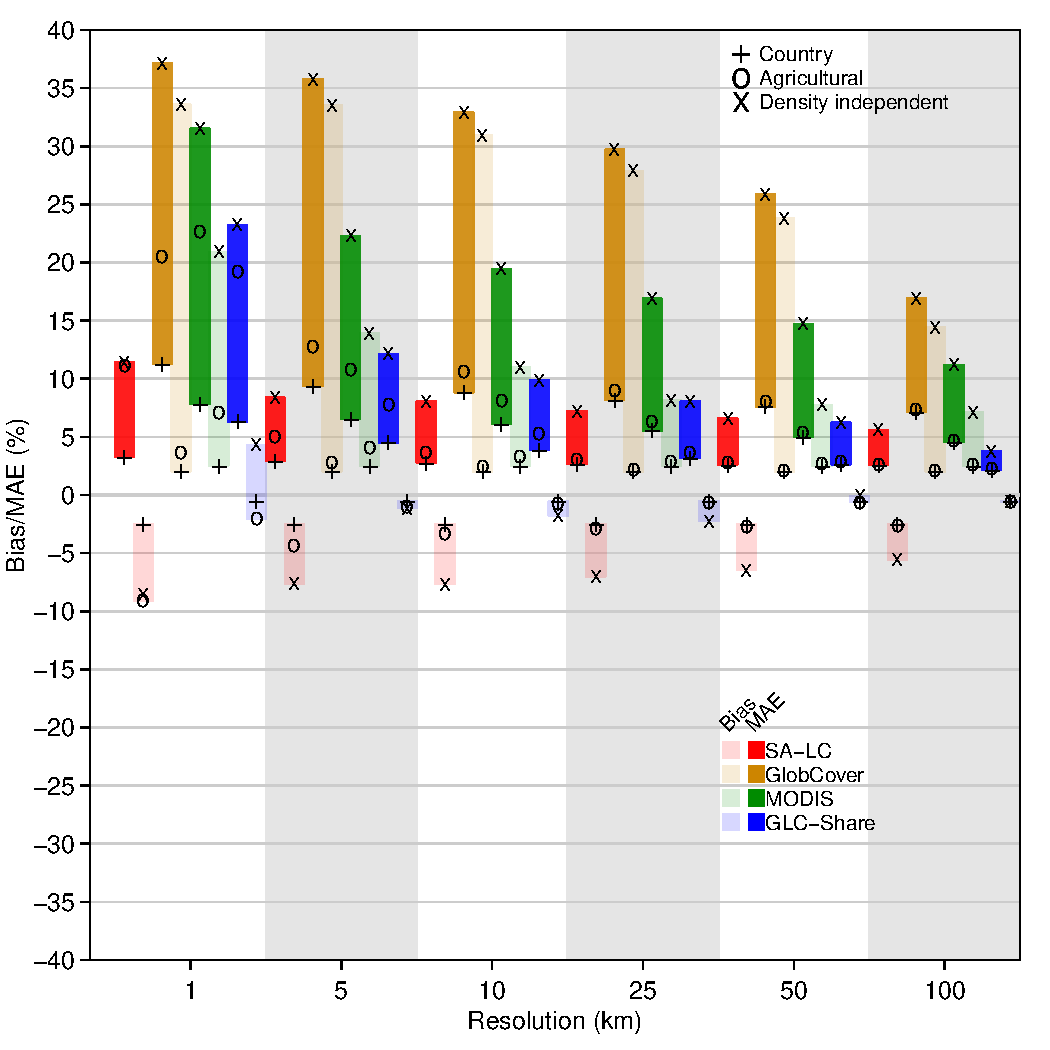
\includegraphics[width = 7cm]{figures/cropland_bias_region.pdf} 
%     \vspace{-3cm}
      \caption{A comparison of three alternate methods for calculating bias and accuracy (mean absolute error): as a straight average across the entire country, averaged over agricultural areas only (the union of areas defined as having $>$0.5\% cropland cover in the reference map and each test map), and independent of cropland density, wherein the mean bias/MAE values for each of 20 cropland cover classes (representing 5\% increments of cover 0\% to 100\% defined by the reference map) were calculated and then averaged.}
      \label{fig:default}
\end{figure}

%% latex table generated in R 3.4.1 by xtable 1.8-2 package
% Sun Aug 27 16:09:11 2017
\begin{longtable}{lllrrrrrr}
\caption{Biases and mean absolute errors (MAE) in cropland maps relative to the 2011 reference map for each aggregation scale calculated over the entire country, for the union of agricultural regions (cropland $>$ 0), and as density independent means, wherein the mean bias/MAE values for each of 20 cropland cover classes (representing 5\% increments of cover 0\% to 100\% defined by the reference map) were calculated and then averaged.} \\ 
  \hline
Region & Metric & Map & 1 km & 5 km & 10 km & 25 km & 50 km & 100 km \\ 
  \hline
Country & Bias & SA-LC & -2.5 & -2.5 & -2.5 & -2.5 & -2.5 & -2.5 \\ 
  Country & Bias & GlobCover & 2.0 & 2.0 & 2.0 & 2.0 & 2.0 & 2.0 \\ 
  Country & Bias & MODIS & 2.5 & 2.5 & 2.5 & 2.5 & 2.5 & 2.5 \\ 
  Country & Bias & GLC-Share & -0.6 & -0.6 & -0.6 & -0.6 & -0.6 & -0.6 \\ 
  Country & MAE & SA-LC & 3.3 & 2.9 & 2.8 & 2.7 & 2.6 & 2.6 \\ 
  Country & MAE & GlobCover & 11.3 & 9.4 & 8.8 & 8.2 & 7.6 & 7.2 \\ 
  Country & MAE & MODIS & 7.8 & 6.5 & 6.1 & 5.6 & 5.0 & 4.6 \\ 
  Country & MAE & GLC-Share & 6.3 & 4.5 & 3.9 & 3.2 & 2.6 & 2.2 \\ 
  Agricultural & Bias & SA-LC & -9.1 & -4.3 & -3.3 & -2.9 & -2.7 & -2.6 \\ 
  Agricultural & Bias & GlobCover & 3.7 & 2.8 & 2.5 & 2.2 & 2.1 & 2.1 \\ 
  Agricultural & Bias & MODIS & 7.1 & 4.1 & 3.4 & 2.9 & 2.7 & 2.6 \\ 
  Agricultural & Bias & GLC-Share & -2.0 & -1.0 & -0.8 & -0.6 & -0.6 & -0.6 \\ 
  Agricultural & MAE & SA-LC & 11.1 & 5.0 & 3.7 & 3.0 & 2.8 & 2.6 \\ 
  Agricultural & MAE & GlobCover & 20.5 & 12.8 & 10.7 & 9.0 & 8.1 & 7.3 \\ 
  Agricultural & MAE & MODIS & 22.7 & 10.8 & 8.2 & 6.3 & 5.4 & 4.7 \\ 
  Agricultural & MAE & GLC-Share & 19.2 & 7.8 & 5.3 & 3.7 & 2.9 & 2.2 \\ 
  Density independent & Bias & SA-LC & -8.6 & -7.6 & -7.7 & -7.0 & -6.5 & -5.5 \\ 
  Density independent & Bias & GlobCover & 33.6 & 33.5 & 30.9 & 27.9 & 23.8 & 14.4 \\ 
  Density independent & Bias & MODIS & 20.9 & 13.9 & 11.0 & 8.1 & 7.7 & 7.1 \\ 
  Density independent & Bias & GLC-Share & 4.3 & -1.1 & -1.8 & -2.3 & -0.1 & -0.6 \\ 
  Density independent & MAE & SA-LC & 11.4 & 8.4 & 8.1 & 7.2 & 6.6 & 5.6 \\ 
  Density independent & MAE & GlobCover & 37.1 & 35.8 & 32.9 & 29.7 & 25.9 & 16.9 \\ 
  Density independent & MAE & MODIS & 31.5 & 22.3 & 19.4 & 16.9 & 14.7 & 11.2 \\ 
  Density independent & MAE & GLC-Share & 23.2 & 12.1 & 9.9 & 8.1 & 6.2 & 3.8 \\ 
   \hline
\hline
\end{longtable}

%% latex table generated in R 3.4.1 by xtable 1.8-2 package
% Sun Aug 27 16:11:21 2017
\begin{longtable}{lllrrrrrr}
\caption{Biases and mean absolute errors (MAE) in cropland maps relative to the 2007 reference map for each aggregation scale calculated over the entire country, for the union of agricultural regions, and as density independent means, wherein the mean bias/MAE values for each of 20 cropland cover classes (representing 5\% increments of cover 0\% to 100\% defined by the reference map) were calculated and then averaged.} \\ 
  \hline
Region & Metric & Map & 1 km & 5 km & 10 km & 25 km & 50 km & 100 km \\ 
  \hline
Country & Bias & SA-LC & -2.9 & -2.9 & -2.9 & -2.9 & -2.9 & -2.9 \\ 
  Country & Bias & GlobCover & 1.7 & 1.7 & 1.7 & 1.7 & 1.7 & 1.7 \\ 
  Country & Bias & MODIS & 2.2 & 2.2 & 2.2 & 2.2 & 2.2 & 2.2 \\ 
  Country & Bias & GLC-Share & -0.9 & -0.9 & -0.9 & -0.9 & -0.9 & -0.9 \\ 
  Country & MAE & SA-LC & 3.0 & 2.9 & 2.9 & 2.9 & 2.9 & 2.9 \\ 
  Country & MAE & GlobCover & 11.3 & 9.4 & 8.9 & 8.2 & 7.7 & 7.2 \\ 
  Country & MAE & MODIS & 7.7 & 6.4 & 6.0 & 5.5 & 5.0 & 4.6 \\ 
  Country & MAE & GLC-Share & 6.2 & 4.4 & 3.8 & 3.1 & 2.6 & 2.2 \\ 
  Agricultural & Bias & SA-LC & -9.9 & -4.9 & -3.8 & -3.2 & -3.1 & -2.9 \\ 
  Agricultural & Bias & GlobCover & 3.1 & 2.3 & 2.0 & 1.9 & 1.8 & 1.7 \\ 
  Agricultural & Bias & MODIS & 6.4 & 3.6 & 2.9 & 2.5 & 2.3 & 2.2 \\ 
  Agricultural & Bias & GLC-Share & -2.8 & -1.6 & -1.2 & -1.0 & -1.0 & -0.9 \\ 
  Agricultural & MAE & SA-LC & 10.4 & 5.0 & 3.9 & 3.3 & 3.1 & 3.0 \\ 
  Agricultural & MAE & GlobCover & 20.6 & 12.8 & 10.7 & 9.1 & 8.1 & 7.4 \\ 
  Agricultural & MAE & MODIS & 22.6 & 10.6 & 8.0 & 6.2 & 5.3 & 4.7 \\ 
  Agricultural & MAE & GLC-Share & 19.2 & 7.7 & 5.2 & 3.6 & 2.8 & 2.2 \\ 
  Density independent & Bias & SA-LC & -9.9 & -8.5 & -8.4 & -7.4 & -6.9 & -6.6 \\ 
  Density independent & Bias & GlobCover & 33.8 & 33.8 & 31.2 & 27.4 & 21.6 & 14.8 \\ 
  Density independent & Bias & MODIS & 20.8 & 13.3 & 10.5 & 7.0 & 6.9 & 7.0 \\ 
  Density independent & Bias & GLC-Share & 3.8 & -1.8 & -2.5 & -2.8 & -0.8 & -1.5 \\ 
  Density independent & MAE & SA-LC & 10.5 & 8.6 & 8.4 & 7.4 & 6.9 & 6.6 \\ 
  Density independent & MAE & GlobCover & 37.4 & 36.1 & 33.2 & 29.3 & 24.0 & 17.4 \\ 
  Density independent & MAE & MODIS & 31.7 & 22.2 & 19.5 & 17.2 & 14.5 & 11.6 \\ 
  Density independent & MAE & GLC-Share & 23.3 & 12.0 & 9.8 & 8.2 & 5.9 & 3.9 \\ 
   \hline
\hline
\end{longtable}


\begin{figure}[!ht]
  \centering
     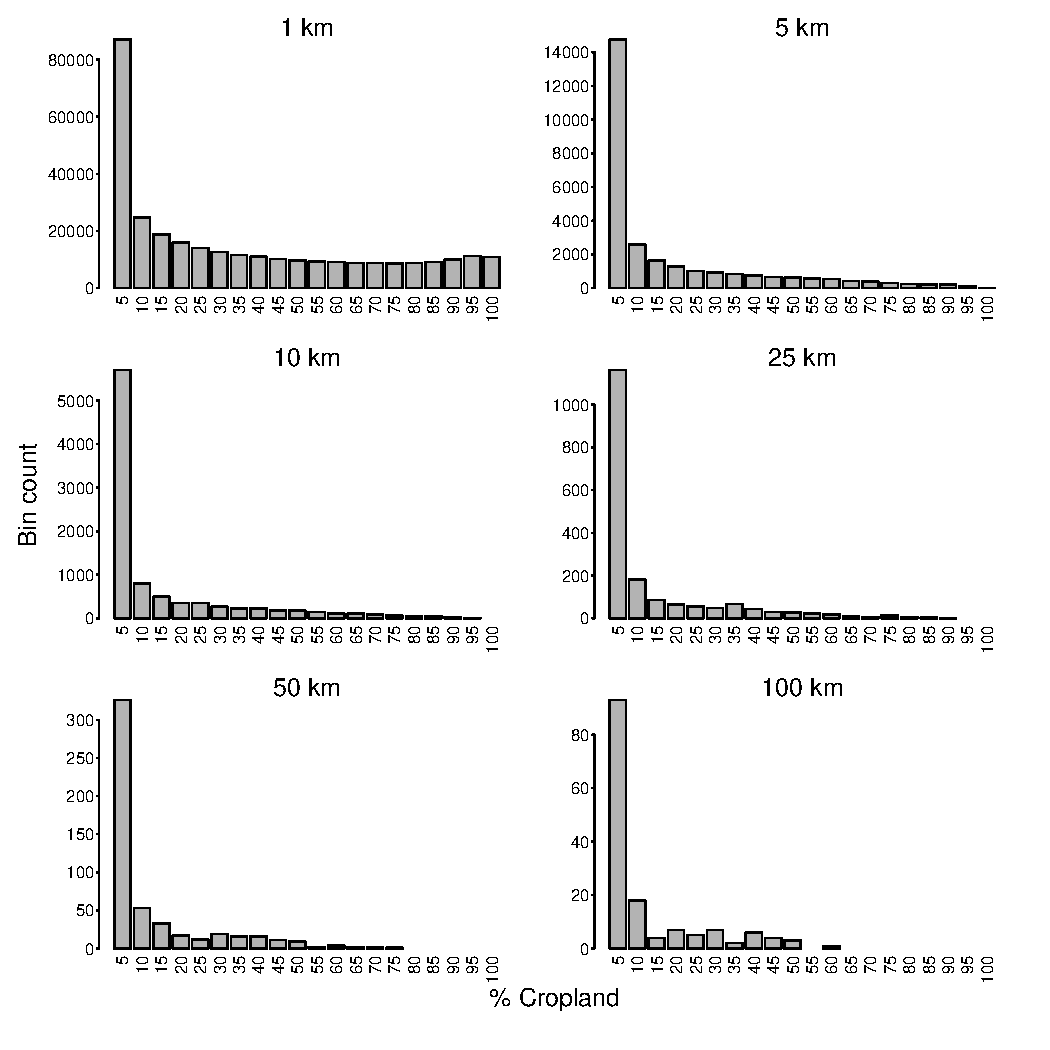
\includegraphics[width = 12cm]{figures/cropland_bins.pdf} 
%     \vspace{-3cm}
      \caption{Number of cells within each cropland density bin at each scale of aggregation, where bins represent 5\% increments of cropland cover (values on x-axis provide the upper limit of each bin). Bin values were based on the 2011 reference map, excluding areas with $<$0.5\% cropland.}
      \label{fig:default}
\end{figure}

We used magisterial district boundaries for South Africa (Fig. 5) to extract absolute residual values for agricultural areas ($>$0.5\% cropland cover) and 2011 reference cropland density values, the means of which respectively served as the response and predictor in the generalized additive model \cite{wood_mgcv:_2001} analysis (main text). 


\begin{figure}[!ht]
  \centering
     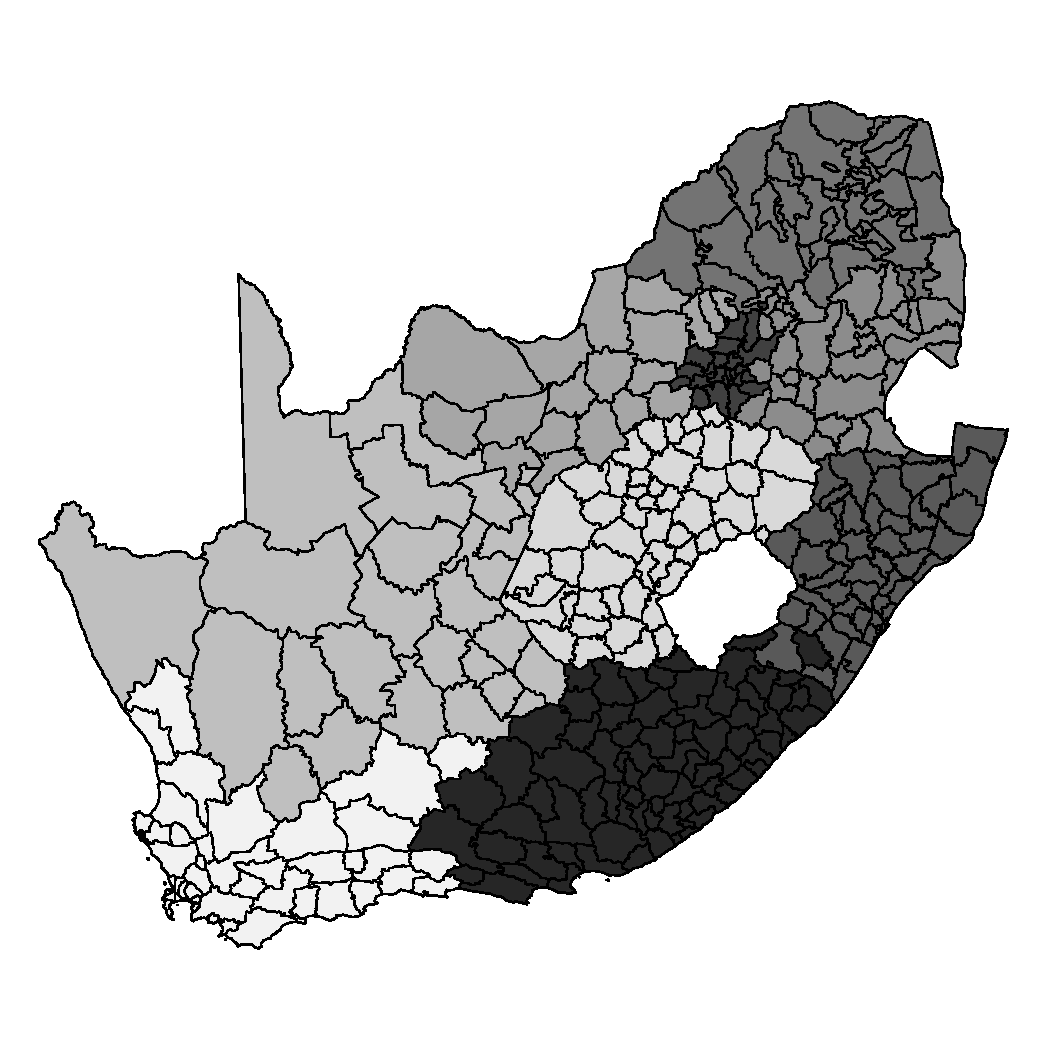
\includegraphics[scale = 0.7]{figures/md_map.pdf} 
%     \vspace{-3cm}
      \caption{South Africa's magisterial districts.}
      \label{fig:default}
\end{figure}

\clearpage
\section{\large Carbon analysis}

To calculate carbon stocks using the method of Ruesch and Gibbs \cite{ruesch_new_2008}, we simplified their landcover-specific carbon density classes into six categories, based on the similarity of their class types and the fact that they had the same assigned carbon densities. Other classes were dropped because of their low level of, or lack of, occurrence. The class adjustments were as follows:

\begin{itemize}
\item Classes 1, 3, 6, 8 corresponding to broadleaf and mixed forests were reduced to a single forest class.
\item Classes 4 and 5 (needleaf forests) were dropped. 
\item Classes 9, 10, 17 (secondary forests, forest/cropland mosaic) where merged to a single secondary forest class.
\item Classes 20-23 (water, snow, ice, built-up areas) were dropped.
\item Class 19 (bare areas) was dropped.
\end{itemize}

All other classes (cropland, shrubland, spare vegetation) were retained. Each of these classes has a specific carbon density according to the ecofloristic zone it is found in, of which there are 10 for Africa (Zones 6-9 and 10-15; see \cite{ruesch_new_2008}). We calculated the area of each ecofloristic zone using their polygon boundary maps\footnote{available from cdiac.ornl.gov/ftp/global\_carbon/ecofloristic\_zones.zip}. For each of the simplified cover classes, we then calculated the mean ecofloristic zone carbon density value, weighted by ecofloristic zone area. We used these values to generate the different carbon maps, as described in the main text.  

Maps of the mean residual differences between the reference map and each of the 5 derived carbon maps for each test map are shown in Figure 6. Table 3 provides the bias and mean absolute errors for the different carbon maps and how they vary with scale.  

\begin{figure}[!ht]
  \centering
     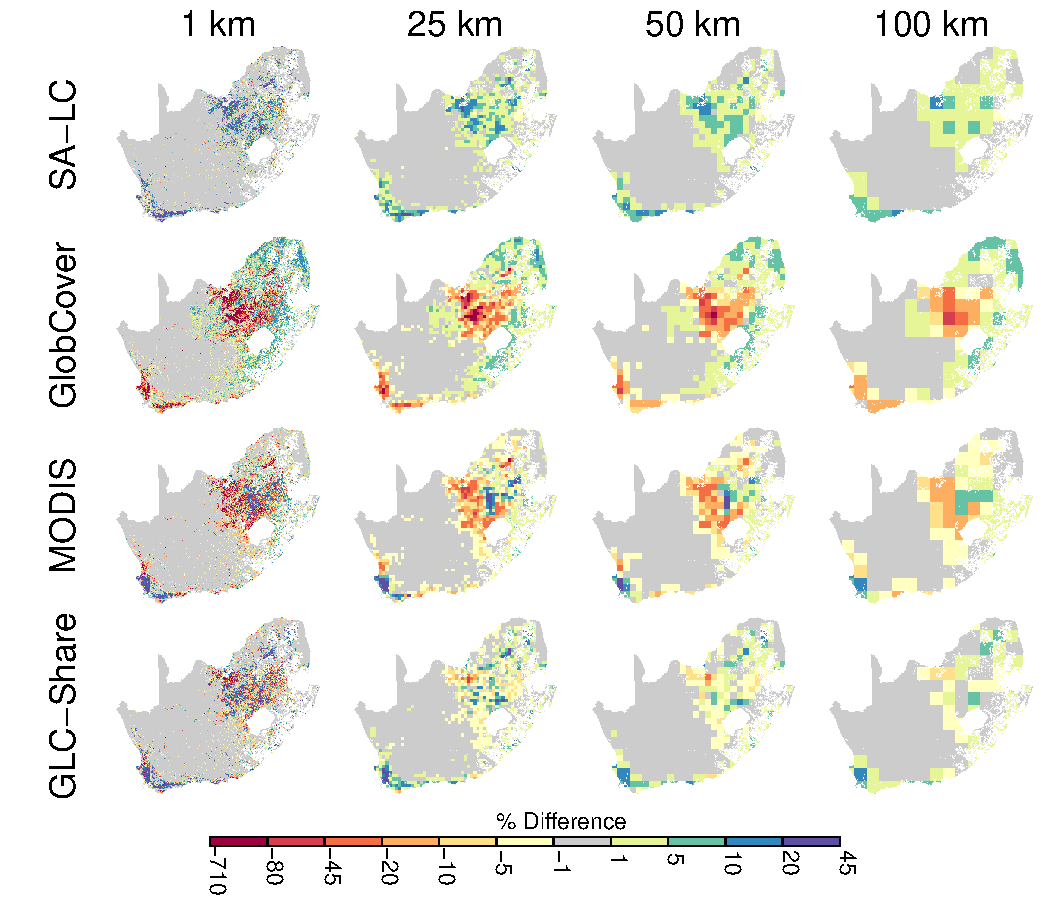
\includegraphics[width = 12cm]{figures/carbon_bias_map.pdf} 
%     \vspace{-3cm}
      \caption{Spatial patterns of error (averaged across all five different possible cover types adjacent to cropland) in carbon stock estimates. }
      \label{fig:default}
\end{figure}

%% latex table generated in R 3.2.1 by xtable 1.7-4 package
% Fri Oct 16 23:40:37 2015
\begin{table}[ht]
\centering
\caption{Percent differences in total carbon stock estimates calculated from the reference maps and from each of the four cropland maps. Differences are evaluated for total carbon estimates either at the country scale or over just the agricultural regions (cropland $>$0.05\%), using the carbon densities of 5 different cover types to provide the values for the non-agricultural portions of each pixel (cover types indicated by column names).} 
\begin{tabular}{llrrrrr}
  \hline
Region & Map & Forest & Secondary & Shrubland & Grassland & Sparse \\ 
  \hline
Country & SA-LC & 2.6 & 2.5 & 2.5 & 0.1 & -2.1 \\ 
  Country & GlobCover & -2.1 & -2.0 & -2.0 & -0.1 & 1.7 \\ 
  Country & MODIS & -2.6 & -2.5 & -2.5 & -0.1 & 2.1 \\ 
  Country & GeoWiki & 0.6 & 0.5 & 0.5 & 0.0 & -0.5 \\ 
  Agricultural & SA-LC & -2.0 & -2.7 & -2.8 & -10.6 & -14.9 \\ 
  Agricultural & GlobCover & -161.9 & -156.3 & -155.5 & -95.9 & -63.6 \\ 
  Agricultural & MODIS & -1.6 & -0.8 & -0.7 & 8.4 & 13.3 \\ 
  Agricultural & GeoWiki & 7.7 & 7.3 & 7.2 & 2.9 & 0.5 \\ 
   \hline
\end{tabular}
\end{table}


\FloatBarrier
% latex table generated in R 3.4.1 by xtable 1.8-2 package
% Fri Sep  1 12:55:34 2017
\begin{longtable}{lllrrrrrr}
\caption{Biases and mean absolute errors, weighted by reference cropland density, for each of the test maps across aggregation scales and each possible landcover type sharing the pixel with cropland.} \\ 
  \hline
Metric & Map & Cover & 1 km & 5 km & 10 km & 25 km & 50 km & 100 km \\ 
  \hline
Bias & SA-LC & All & 10.9 & 9.6 & 8.2 & 6.5 & 5.0 & 4.2 \\ 
  Bias & GlobCover & All & -123.4 & -47.6 & -35.9 & -24.8 & -17.4 & -12.3 \\ 
  Bias & MODIS & All & -66.0 & -17.6 & -12.0 & -8.3 & -6.2 & -4.1 \\ 
  Bias & GLC-Share & All & -20.4 & 2.1 & 2.3 & 1.3 & 0.3 & 0.5 \\ 
  Bias & SA-LC & Forest & 22.7 & 19.7 & 16.9 & 13.3 & 10.4 & 9.0 \\ 
  Bias & GlobCover & Forest & -276.2 & -98.3 & -73.3 & -50.2 & -35.5 & -25.4 \\ 
  Bias & MODIS & Forest & -146.5 & -36.1 & -24.5 & -17.0 & -12.9 & -8.8 \\ 
  Bias & GLC-Share & Forest & -46.1 & 4.3 & 4.6 & 2.7 & 0.6 & 1.0 \\ 
  Bias & SA-LC & Secondary & 18.4 & 16.7 & 14.6 & 11.8 & 9.5 & 8.2 \\ 
  Bias & GlobCover & Secondary & -186.3 & -79.3 & -61.2 & -43.8 & -31.7 & -23.2 \\ 
  Bias & MODIS & Secondary & -101.0 & -30.6 & -21.5 & -15.2 & -11.7 & -8.0 \\ 
  Bias & GLC-Share & Secondary & -30.5 & 3.4 & 3.7 & 2.2 & 0.6 & 0.9 \\ 
  Bias & SA-LC & Shrubland & 17.9 & 16.4 & 14.3 & 11.6 & 9.4 & 8.1 \\ 
  Bias & GlobCover & Shrubland & -178.2 & -77.1 & -59.8 & -42.9 & -31.2 & -22.9 \\ 
  Bias & MODIS & Shrubland & -96.8 & -29.9 & -21.1 & -15.0 & -11.5 & -7.9 \\ 
  Bias & GLC-Share & Shrubland & -29.2 & 3.3 & 3.6 & 2.2 & 0.6 & 0.9 \\ 
  Bias & SA-LC & Grassland & 0.3 & 0.3 & 0.3 & 0.3 & 0.2 & 0.2 \\ 
  Bias & GlobCover & Grassland & -1.9 & -1.2 & -1.1 & -0.9 & -0.8 & -0.6 \\ 
  Bias & MODIS & Grassland & -1.1 & -0.6 & -0.5 & -0.4 & -0.3 & -0.2 \\ 
  Bias & GLC-Share & Grassland & -0.3 & 0.0 & 0.1 & 0.0 & 0.0 & 0.0 \\ 
  Bias & SA-LC & Sparse & -4.6 & -5.2 & -5.1 & -4.8 & -4.6 & -4.4 \\ 
  Bias & GlobCover & Sparse & 25.4 & 18.1 & 16.1 & 13.9 & 12.2 & 10.5 \\ 
  Bias & MODIS & Sparse & 15.4 & 9.1 & 7.6 & 6.3 & 5.5 & 4.4 \\ 
  Bias & GLC-Share & Sparse & 4.0 & -0.3 & -0.6 & -0.5 & -0.3 & -0.4 \\ 
  MAE & SA-LC & All & 19.2 & 12.5 & 10.7 & 8.6 & 6.9 & 6.0 \\ 
  MAE & GlobCover & All & 134.9 & 56.2 & 43.8 & 31.9 & 23.9 & 18.2 \\ 
  MAE & MODIS & All & 84.8 & 33.2 & 26.2 & 19.9 & 14.9 & 11.4 \\ 
  MAE & GLC-Share & All & 47.3 & 17.9 & 12.8 & 8.8 & 5.8 & 3.9 \\ 
  MAE & SA-LC & Forest & 34.8 & 21.0 & 17.5 & 13.6 & 10.6 & 9.1 \\ 
  MAE & GlobCover & Forest & 278.2 & 100.3 & 75.3 & 52.4 & 37.6 & 27.7 \\ 
  MAE & MODIS & Forest & 168.6 & 56.2 & 42.9 & 31.6 & 22.9 & 17.1 \\ 
  MAE & GLC-Share & Forest & 90.5 & 29.9 & 20.9 & 14.0 & 8.9 & 5.8 \\ 
  MAE & SA-LC & Secondary & 27.4 & 17.9 & 15.2 & 12.1 & 9.6 & 8.3 \\ 
  MAE & GlobCover & Secondary & 188.1 & 81.1 & 63.1 & 45.7 & 33.8 & 25.3 \\ 
  MAE & MODIS & Secondary & 118.9 & 47.6 & 37.3 & 28.1 & 20.8 & 15.7 \\ 
  MAE & GLC-Share & Secondary & 66.6 & 25.5 & 18.1 & 12.4 & 8.0 & 5.4 \\ 
  MAE & SA-LC & Shrubland & 26.6 & 17.6 & 14.9 & 11.9 & 9.5 & 8.2 \\ 
  MAE & GlobCover & Shrubland & 179.9 & 79.0 & 61.7 & 44.9 & 33.2 & 24.9 \\ 
  MAE & MODIS & Shrubland & 114.2 & 46.6 & 36.6 & 27.7 & 20.5 & 15.5 \\ 
  MAE & GLC-Share & Shrubland & 64.3 & 24.9 & 17.8 & 12.2 & 7.9 & 5.3 \\ 
  MAE & SA-LC & Grassland & 0.4 & 0.4 & 0.3 & 0.3 & 0.2 & 0.2 \\ 
  MAE & GlobCover & Grassland & 1.9 & 1.3 & 1.1 & 1.0 & 0.8 & 0.7 \\ 
  MAE & MODIS & Grassland & 1.4 & 0.9 & 0.8 & 0.7 & 0.6 & 0.5 \\ 
  MAE & GLC-Share & Grassland & 0.9 & 0.5 & 0.4 & 0.3 & 0.2 & 0.2 \\ 
  MAE & SA-LC & Sparse & 6.7 & 5.8 & 5.4 & 4.9 & 4.7 & 4.4 \\ 
  MAE & GlobCover & Sparse & 26.4 & 19.6 & 17.7 & 15.7 & 14.0 & 12.3 \\ 
  MAE & MODIS & Sparse & 20.7 & 14.9 & 13.3 & 11.5 & 9.7 & 8.3 \\ 
  MAE & GLC-Share & Sparse & 14.1 & 8.4 & 6.6 & 5.1 & 3.9 & 2.9 \\ 
   \hline
\hline
\end{longtable}


\clearpage
\section{\large Gridded maize yield and production}

For our crop yield and production analysis, we followed several steps to create the gridded yield and crop production maps. First, we calibrated cropland percentage maps so that they matched total cropland areas reported for coarser administrative units, following methods set out by Ramankutty et al \cite{ramankutty_farming_2008}: 

\begin{enumerate}
 \item We extracted the 2011 reference percentages within each of South Africa's 9 provinces (the same units used by Ramankutty et al \cite{ramankutty_farming_2008}, converted these to proportions and summed them to calculate the ``reported'' cropland areas for each province. We did the same to calculate provincial cropland areas for each test map;  
  \item We divided the ``reported'' provincial cropland area estimates by provincial areas to calculate \emph{rpcf}, the reference provincial cropland fractions, and then did the same with test map provincial cropland areas to calculate \emph{tpcf}, the test map provincial cropland fractions; 
  \item A province-specific correction factor \emph{upcf} (\emph{rpcf/tpcf}) was then calculated and applied to each testmap cropland fraction (\emph{tcf}) in each pixel (x, y):

  \begin{equation}  
    \textrm{tcfa}_{x,y} = \textrm{upcf}_{x,y} * \textrm{tcf}_{x,y}
  \end{equation}

Yielding \emph{tcfa}, the calibrated test map cropland fraction.  
\end{enumerate}

The differences between the reference map cropland fraction and \emph{tfca} are shown in Figure 7 (where they were adjusted back to percentages), while Table 4 provides the corresponding bias and accuracy values (MAE).

We then used \emph{tcfa}, per Monfreda et al \cite{monfreda_farming_2008}, to disaggregate magisterial district-level reported maize yields and harvested areas \cite{statistics_south_africa_building_2007}, according to the following steps: 

\begin{enumerate}
  \item We first disaggregated maize yields using the following formula: 
  
  \begin{equation}
  \textrm{fcrop}_{x,y} = \textrm{tfca}_{x,y}\frac{\textrm{cmda}}{\textrm{tmda}}
  \end{equation}
  
  Where \emph{fcrop} is the fraction of each cell in each district harvested for maize, \emph{cmda} is the district-reported harvested area for maize, and \emph{tmda} is the total area of the magisterial district;
  \item The reported maize yield for each magisterial district was then assigned to each pixel in \emph{fcrop} in the district having non-zero maize harvested areas;
  \item Production estimates were calculated by multiplying yield and harvested areas.
\end{enumerate}

The maps of differences between reference-derived yield and production maps and those based on the test maps are shown in Figures 8 and 9, where the values were normalized to the country mean yield or production (calculated from the reference map).  Table 5 presents the bias and accuracy values for each reference-test comparison of gridded yield and production estimates, giving both the cropland density-weighted variants of bias and accuracy, and for comparison the same values calculated as straight averages within agricultural pixels (i.e. pixels in the reference or test map having $.$0.5\% cropland). In the former variant, yields show relatively much less bias than in the latter, where large yield biases were driven by the discrepancies in the low cropland density regions in the center of the country. In contrast, the density-weighted measures reveal large production biases, whereas the unweighted agricultural region measures show no bias in production estimates.  The density-weighted variant shows that error scales with cropland cover, as seen in Figure 2 in the main text. 

\begin{figure}[ht]
  \centering
     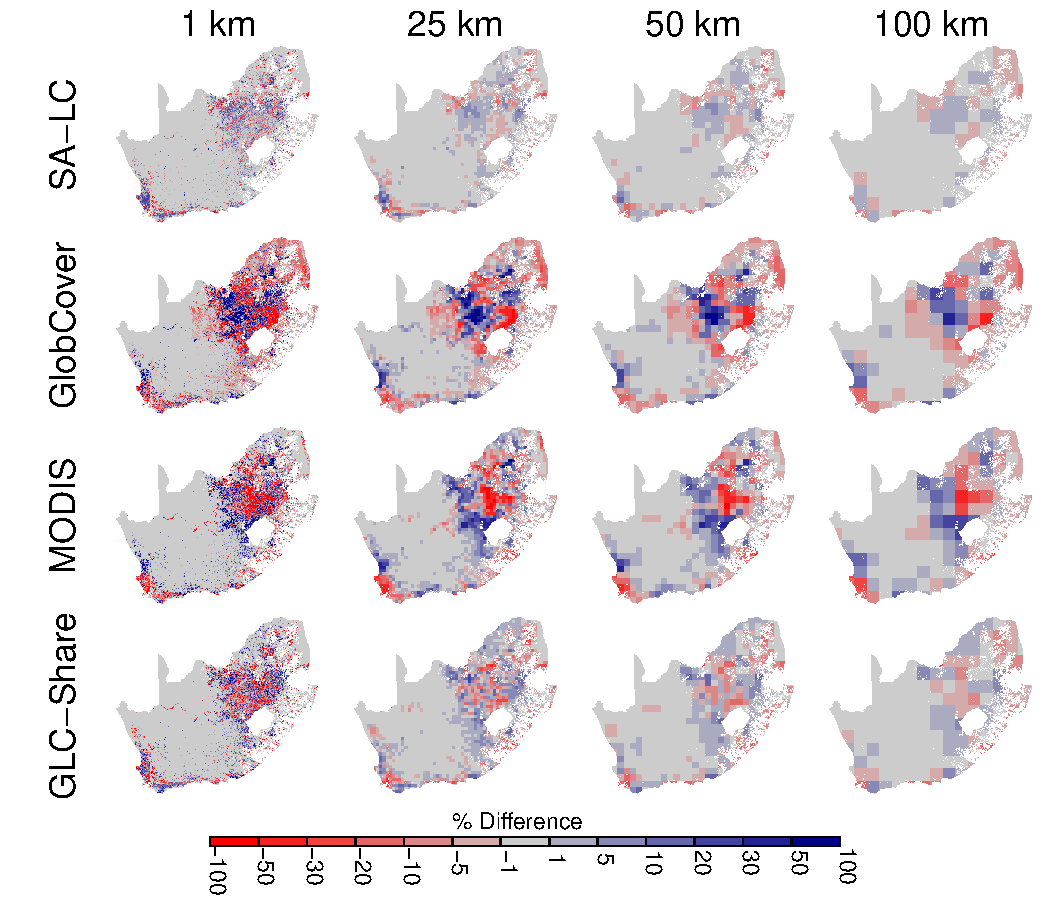
\includegraphics[width = 12cm]{figures/cropland_adj_bias_map2.pdf} 
      \caption{Errors in cropland maps adjusted using provincial cropland area statistics.}
      \label{fig:default}
\end{figure}

\FloatBarrier
% latex table generated in R 3.4.1 by xtable 1.8-2 package
% Fri Sep  1 14:57:19 2017
\begin{longtable}{llrrrrrr}
\caption{Bias and mean absolute errors (MAE) in statistically constrained cropland maps across aggregation scales, weighted by density of cropland cover in the reference map. } \\ 
  \hline
Metric & Map & 1 km & 5 km & 10 km & 25 km & 50 km & 100 km \\ 
  \hline
Bias & GLC-Share & 9.7 & 1.1 & 0.6 & 0.4 & 0.5 & 0.1 \\ 
  Bias & GlobCover & 34.5 & 18.3 & 14.5 & 10.6 & 7.6 & 4.6 \\ 
  Bias & MODIS & 17.8 & 5.5 & 3.2 & 1.3 & 0.1 & -1.3 \\ 
  Bias & SA-LC & 6.6 & 2.7 & 2.1 & 1.6 & 1.1 & 0.6 \\ 
  Accuracy & GLC-Share & 23.8 & 12.6 & 9.4 & 6.8 & 4.8 & 3.0 \\ 
  Accuracy & GlobCover & 42.3 & 27.3 & 23.3 & 18.8 & 15.6 & 11.2 \\ 
  Accuracy & MODIS & 33.8 & 21.5 & 18.4 & 15.3 & 12.7 & 10.6 \\ 
  Accuracy & SA-LC & 11.4 & 6.0 & 4.7 & 3.7 & 2.8 & 1.9 \\ 
   \hline
\hline
\end{longtable}


\clearpage
\begin{figure}[ht]
  \centering
     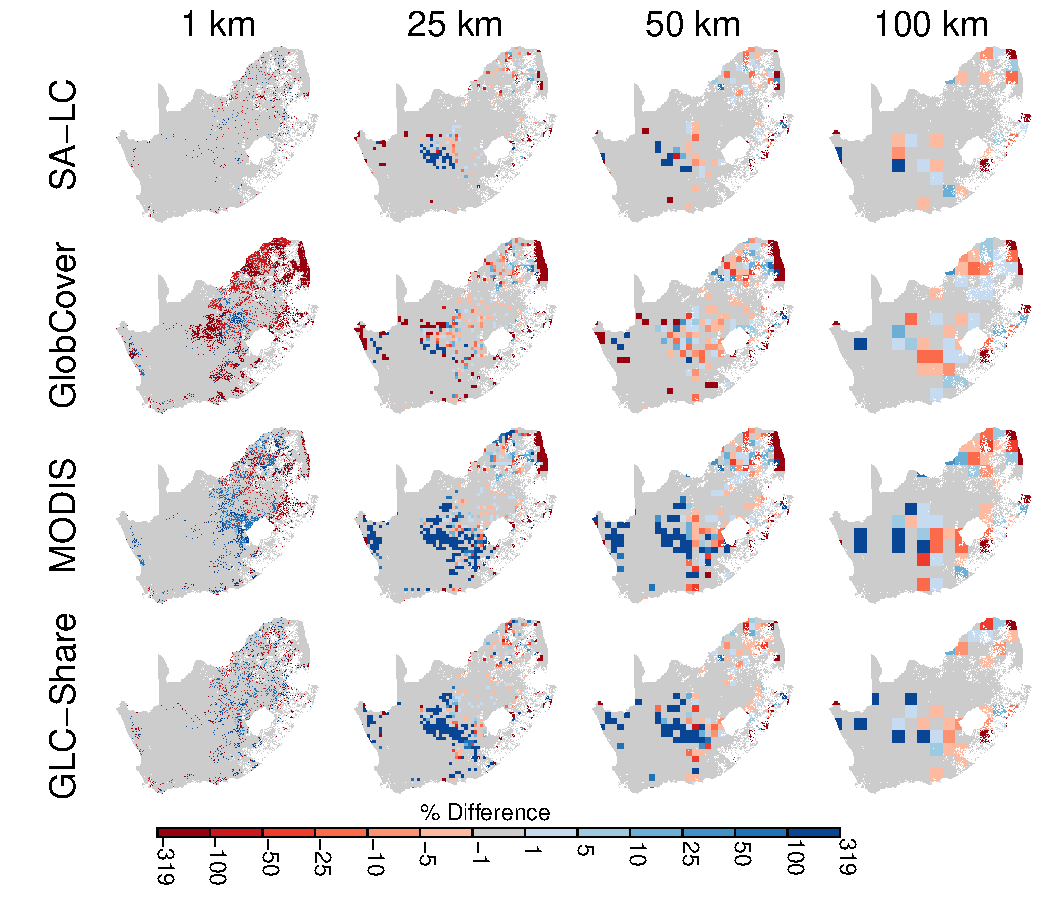
\includegraphics[width = 12cm]{figures/yld_bias_map.pdf} 
      \caption{Errors (normalized to the reference-derived country mean) in disaggregated maize yield estimates.}
      \label{fig:default}
\end{figure}

\begin{figure}[ht]
  \centering
     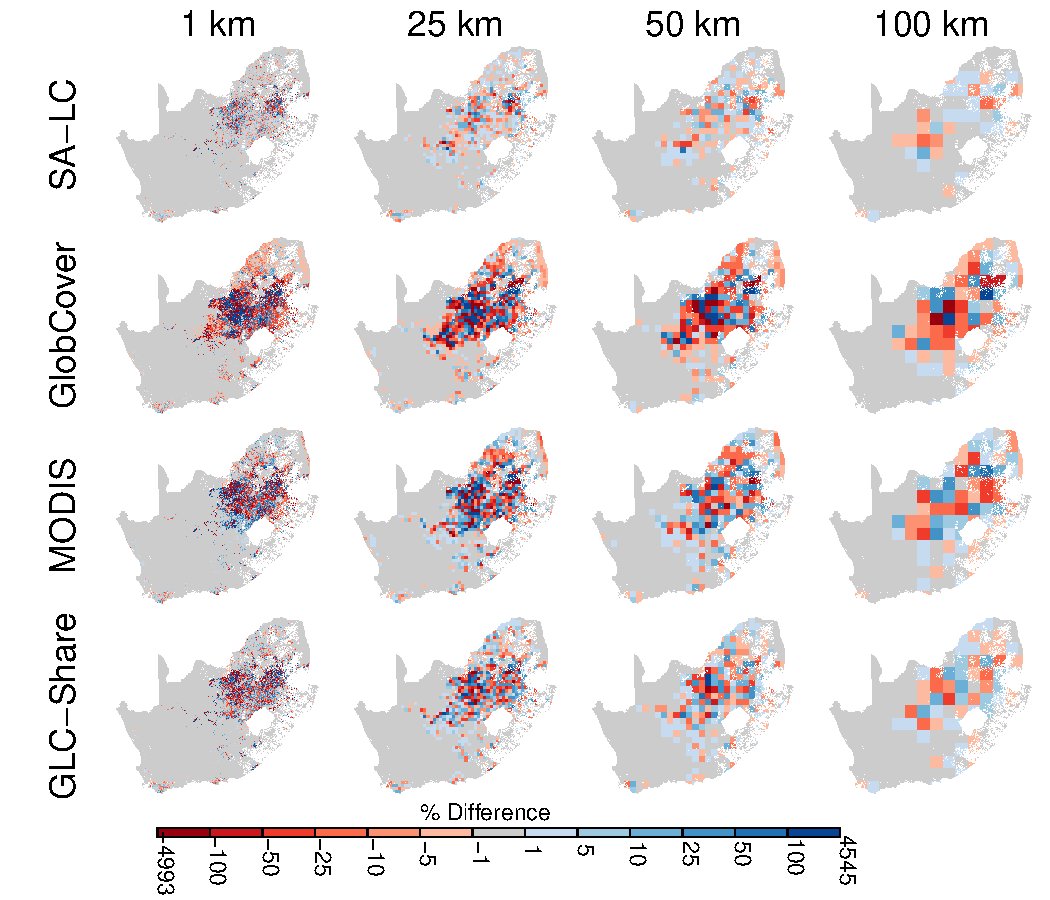
\includegraphics[width = 12cm]{figures/prod_bias_map.pdf} 
      \caption{Errors (normalized to reference-derived country mean) production estimates calculated from disaggregated maize yield and harvested area estimates.}
      \label{fig:default}
\end{figure}

\FloatBarrier
% latex table generated in R 3.4.1 by xtable 1.8-2 package
% Fri Sep  1 15:01:36 2017
\begin{longtable}{llllrrrrrr}
\caption{Biases and mean absolute errors (MAE) in disaggregated maize yield and production (calculated from disaggregated yield and harvested area estimates) maps. Values for both density-weighted and agricultural areas bias and accuracy are presennted. Bias and MAE were normalized to their respective mean values calculated from reference maps.} \\ 
  \hline
Region & Metric & Map & Variable & 1 km & 5 km & 10 km & 25 km & 50 km & 100 km \\ 
  \hline
Density & Bias & SA-LC & Yield & 1.2 & 0.3 & 0.0 & 0.0 & 0.0 & -0.3 \\ 
  Density & Bias & GlobCover & Yield & 9.8 & 0.9 & 0.0 & -0.6 & -0.6 & -0.6 \\ 
  Density & Bias & MODIS & Yield & 19.6 & 8.9 & 5.7 & 3.0 & 1.5 & -0.6 \\ 
  Density & Bias & GLC-Share & Yield & 8.0 & 3.0 & 1.5 & 0.6 & 0.3 & -0.6 \\ 
  Density & Bias & SA-LC & Production & 6.9 & 1.6 & 0.5 & -0.2 & -0.1 & -0.1 \\ 
  Density & Bias & GlobCover & Production & 60.5 & 50.2 & 43.7 & 35.1 & 23.3 & 12.5 \\ 
  Density & Bias & MODIS & Production & 21.9 & 6.0 & 1.8 & -1.8 & -0.9 & -0.5 \\ 
  Density & Bias & GLC-Share & Production & 12.7 & -3.3 & -4.6 & -3.8 & -0.5 & -0.9 \\ 
  Density & MAE & SA-LC & Yield & 1.2 & 0.3 & 0.3 & 0.3 & 0.6 & 0.9 \\ 
  Density & MAE & GlobCover & Yield & 9.8 & 1.2 & 0.9 & 1.5 & 1.8 & 1.8 \\ 
  Density & MAE & MODIS & Yield & 19.6 & 9.2 & 6.2 & 4.5 & 3.9 & 2.4 \\ 
  Density & MAE & GLC-Share & Yield & 8.0 & 3.3 & 1.8 & 1.8 & 1.2 & 1.2 \\ 
  Density & MAE & SA-LC & Production & 19.0 & 14.3 & 11.8 & 8.9 & 5.1 & 2.3 \\ 
  Density & MAE & GlobCover & Production & 95.6 & 102.0 & 100.4 & 88.1 & 65.8 & 46.4 \\ 
  Density & MAE & MODIS & Production & 66.8 & 62.0 & 58.4 & 46.4 & 25.7 & 14.6 \\ 
  Density & MAE & GLC-Share & Production & 47.3 & 43.6 & 37.6 & 29.3 & 19.4 & 7.9 \\ 
  Agricultural & Bias & SA-LC & Yield & -5.1 & -0.3 & 3.0 & 3.6 & 3.6 & 1.5 \\ 
  Agricultural & Bias & GlobCover & Yield & -58.0 & -36.0 & -22.3 & -11.9 & -8.9 & -1.5 \\ 
  Agricultural & Bias & MODIS & Yield & 5.1 & 21.4 & 29.2 & 26.8 & 20.5 & 11.6 \\ 
  Agricultural & Bias & GLC-Share & Yield & 2.4 & 24.4 & 29.5 & 25.3 & 21.4 & 9.8 \\ 
  Agricultural & Bias & SA-LC & Production & 0.0 & -0.1 & -0.1 & -0.1 & -0.0 & 0.0 \\ 
  Agricultural & Bias & GlobCover & Production & 0.0 & -0.1 & 0.0 & 0.1 & 0.3 & 0.3 \\ 
  Agricultural & Bias & MODIS & Production & 0.0 & -0.1 & -0.1 & -0.1 & 0.0 & -0.1 \\ 
  Agricultural & Bias & GLC-Share & Production & 0.0 & 0.1 & 0.0 & 0.0 & 0.1 & 0.1 \\ 
  Agricultural & MAE & SA-LC & Yield & 15.5 & 16.7 & 19.9 & 15.8 & 12.2 & 6.8 \\ 
  Agricultural & MAE & GlobCover & Yield & 71.7 & 48.2 & 38.1 & 23.5 & 17.3 & 6.2 \\ 
  Agricultural & MAE & MODIS & Yield & 55.9 & 51.2 & 50.9 & 44.9 & 38.4 & 20.8 \\ 
  Agricultural & MAE & GLC-Share & Yield & 41.1 & 41.1 & 40.5 & 35.1 & 28.6 & 14.6 \\ 
  Agricultural & MAE & SA-LC & Production & 19.7 & 11.3 & 8.6 & 5.5 & 3.3 & 1.9 \\ 
  Agricultural & MAE & GlobCover & Production & 55.7 & 55.5 & 52.5 & 42.2 & 28.1 & 17.3 \\ 
  Agricultural & MAE & MODIS & Production & 56.0 & 41.3 & 35.6 & 24.9 & 14.1 & 8.4 \\ 
  Agricultural & MAE & GLC-Share & Production & 43.7 & 30.2 & 23.5 & 15.3 & 9.3 & 4.0 \\ 
   \hline
\hline
\end{longtable}


\section{\large Evapotranspiration analysis}
%% latex table generated in R 3.2.1 by xtable 1.7-4 package
% Thu Sep 24 11:01:34 2015
\begin{longtable}{llrr}
\caption{Biases and mean absolute errors (as \%) for evapotranspiration variables derived from a 29-year time series calculated by the VIC model, including the average total ET for the 3 months of the year when ET is highest, the annual mean and the minimum and maximum annual ETs in the time series.} \\ 
  \hline
Variable & Map & Bias & Abs Bias \\ 
  \hline
Peak & GeoWiki & 0.2 & 0.8 \\ 
  Annual Mean & GeoWiki & 0.3 & 0.7 \\ 
  29-year Min & GeoWiki & 0.3 & 0.6 \\ 
  29-year Max & GeoWiki & 0.3 & 0.8 \\ 
  Peak & GlobCover & 0.1 & 1.2 \\ 
  Annual Mean & GlobCover & -0.1 & 1.0 \\ 
  29-year Min & GlobCover & -0.2 & 0.9 \\ 
  29-year Max & GlobCover & 0.2 & 1.2 \\ 
  Peak & MODIS & -0.5 & 0.9 \\ 
  Annual Mean & MODIS & -0.6 & 0.8 \\ 
  29-year Min & MODIS & -0.6 & 0.7 \\ 
  29-year Max & MODIS & -0.5 & 0.8 \\ 
  Peak & SA-LC & 0.3 & 0.7 \\ 
  Annual Mean & SA-LC & 0.5 & 0.6 \\ 
  29-year Min & SA-LC & 0.4 & 0.5 \\ 
  29-year Max & SA-LC & 0.4 & 0.6 \\ 
   \hline
\hline
\end{longtable}

A number of the variables used by the Variable Infiltration Capacity \cite[VIC][]{liang_simple_1994} model are linked to a 0.25$^{\circ}$ resolution, AVHRR-derived landcover map. These include seasonal leaf area index (LAI) phenologies (Fig. 10), as well as other properties such as plant rooting depth and infiltration rates. Landcover properties therefore impact the model's simulation of water balance. To test how landcover map error impacts VIC simulations, we created five new versions of VIC's native landcover scheme, one based on the reference cropland map, and the other four on each of the test maps. For each version, we first reprojected the relevant 25 km cropland map to the geographic coordinate system used by VIC and resampled it to 0.25$^{\circ}$. We then adjusted VIC's landcover scheme by replacing its existing cropland percentages with those from our map, and then proportionally adjusted the remaining cover types in each cell to accommodate the changed cropland amounts. Since LAI is strongly linked to rainfall seasonality in South Africa, which varies between winter (May-August) rainfall in the west and southwest of the country and summer (October-March) rainfall in the east and northeast, we assigned LAI curves that peaked during the winter months to the cover types in the western half of the country, and those peaking in the summer months to the eastern half (Fig. 10). 

\begin{figure}[!ht]
  \centering
     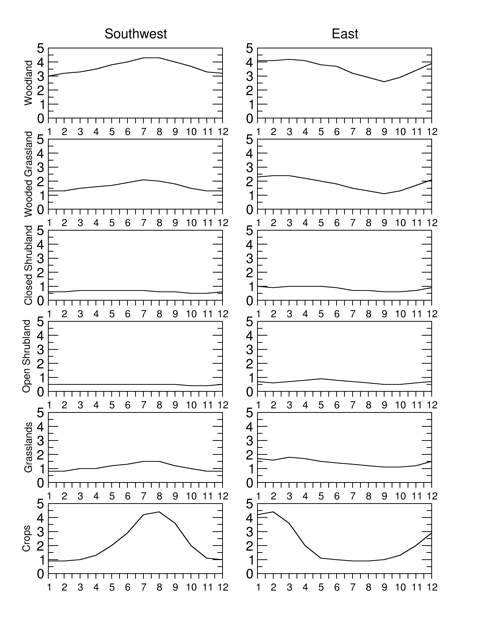
\includegraphics[width = 10cm]{figures/lai_seasonal_cycles.png} 
      \caption{Seasonal LAI curves for different cover types in VIC's landcover scheme, showing the phenologies used for the winter-rainfall portion of the country in the west and southwest (left column), and for the summer rainfall region in the country's easter to northeast (right column). }
      \label{fig:default}
\end{figure}

After making these adjustments, we conducted five different VIC simulations, one for each of the adjusted landcover schemes. The model was run at a daily time step for 28 years, from 1981-2008, from which monthly total evapotranspiration values were extracted.  We calculated from these results the average annual total ET, the maximum and minimum monthly ET observed throughout the entire time series, and the mean ET during the month which on average had the highest ET during the time series. We then found the differences between the reference and test map variants of each of these ET variables, and calculated their bias and MAE values (Fig. 11). The results are similar across the four variables, and we present the difference maps for the mean annual ET comparison in the main text.  

\begin{figure}[ht]
  \centering
     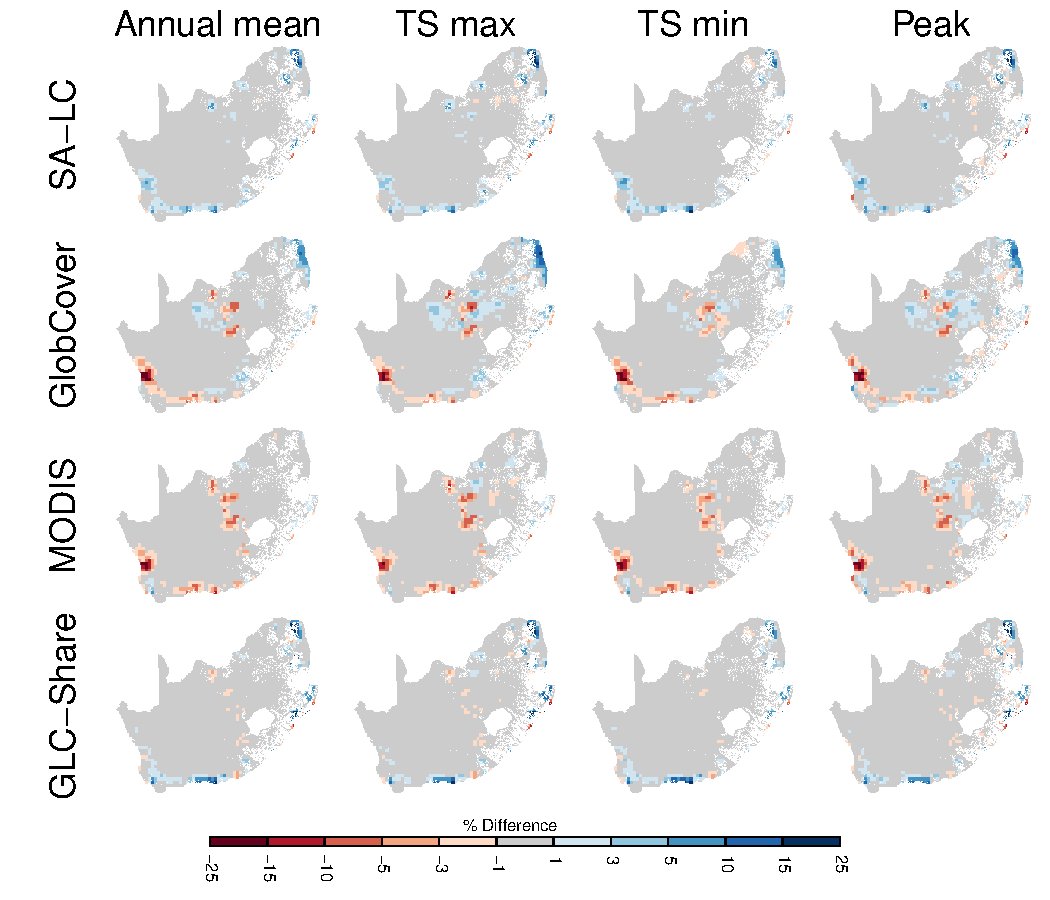
\includegraphics[width = 12cm]{figures/et_bias_map4.pdf} 
      \caption{Maps of error between reference- and test map-derived ET estimates simulated by the VIC model. Four different variants of ET were assessed: annual mean (left column, also presented in Fig. 2 of the main text), the maximum (second column, TS max) and minimum (third column, TS min) ET values observed during the 30 year times, and mean ET during the month in which ET peaks (right column, Peak).}
      \label{fig:default}
\end{figure}


\section{\large Agent-based model assessment}

\subsection{\large Maize production}
The agent-based model simulates household food production using a look-up table that links maize yields to several different variables: planting date; cultivar (open-pollinated or hybrid); soil properties, and weather.  The look-up table itself was based on a series of yield simulations conducted by the DSSAT cropping system model run over 31 years (1979-2010) for a location in the southern Province of Zambia, corresponding to the region where household survey data were collected. The model was run for three dominant soil series\footnote{extracted from a gridded version of the ISRIC-WISE database, available from http://dssat.net/649}, using two open-pollinated and two hybrid cultivars (each pair representing a short- and medium-length growing season variety) whose coefficients were obtained from the inputs files for the PSIMs modeling platform \cite{elliott_parallel_2014}. Each cultivar was simulated under planting dates ranging from October 15th until January 30th, varying by 15 day increments, with row spacing fixed at 90 cm and planting density at 3.7 plants m$^2$, and 5 kg ha$^{-1}$ applied at planting. Models were run using weather data extracted from a bias-corrected version of the Princeton Global Meteorological forcing dataset \cite{sheffield_development_2006,chaney_spatial_2014,estes_changing_2014}.  

\subsection{\large District selection}
For our analysis of how landcover map error impacts agent-based model results, we selected four districts in South Africa which had similar climatic characteristics ($\sim$800 mm annual rainfall) to the region in Zambia where the crop model simulations and household survey data were collected.  These were four contiguous districts along the western border of Lesotho, Clocolan, Ficksburg, Fouriesburg, and Marquard (Fig. 12, top left), which had between 29-45\% of their areas covered by cropland, according to the 2011 reference map (Fig. 12, top right).  

\begin{figure}[!ht]
  \centering
     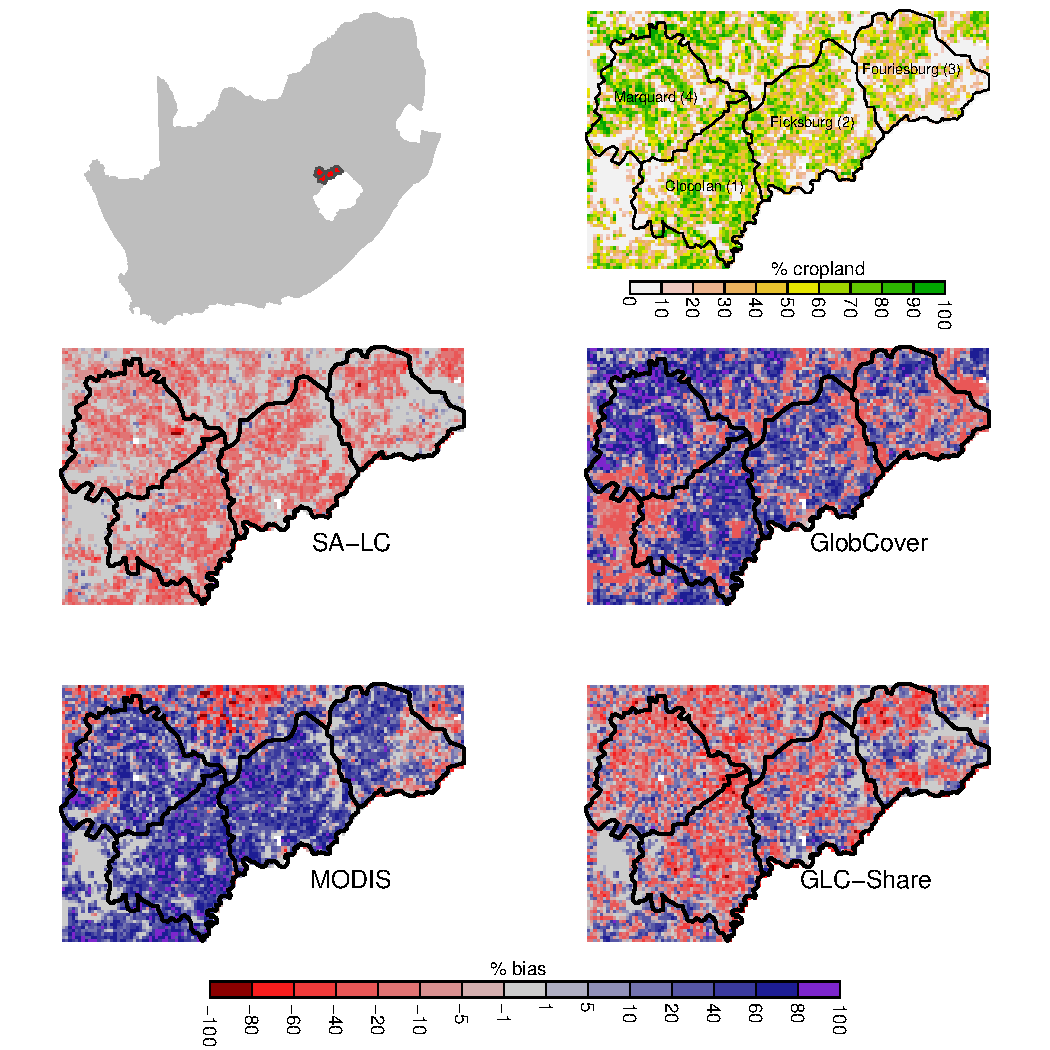
\includegraphics[width = 12cm]{figures/abm-selected-districts.pdf} 
      \caption{The location of the four selected magisterial districts (top left) used in evaluating agent allocation bias, the reference levels of cropland cover within those districts (top right), and the difference in cropland percentage between the reference and each of the four cropland maps (lower four panels). }
      \label{fig:default}
\end{figure}



\FloatBarrier
%\section*{References}
\bibliographystyle{pnas2011} 
{\footnotesize \bibliography{/Users/lestes/Dropbox/publications/full.bib}}
\end{document}  

